\chapter{Smoothing and Gaussian Pyramids}
\label{ch:lesson11}

Chapter~\ref{ch:lesson10} introduced Gaussian blur as one convolution kernel among several. Here we look at \emph{why} blurring matters beyond just ``softening'' an image: it's the key ingredient that makes downsampling safe. That leads directly to the \textbf{Gaussian pyramid} --- a stack of progressively smaller, blurrier versions of an image, used throughout computer vision for multi-scale analysis.

\section{Why downsampling needs blurring first}

Naively shrinking an image by keeping every $k$-th pixel (``nearest-neighbor downsampling'') can produce \textbf{aliasing}: fine periodic detail that oscillates faster than the new pixel spacing can represent folds into a completely different, fake low-frequency pattern. A photo of a brick wall demonstrates this well --- the repeating rows of bricks and mortar lines are exactly the kind of fine, regular detail that aliases badly.

\begin{lstlisting}
factor = 4
naive_downsample = brick_wall[::factor, ::factor]
safe_downsample = cv2.GaussianBlur(brick_wall, (0, 0), sigmaX=factor/2)[::factor, ::factor]
\end{lstlisting}

Figure~\ref{fig:l11-1} shows the difference directly.

\begin{figure}[h]
\centering
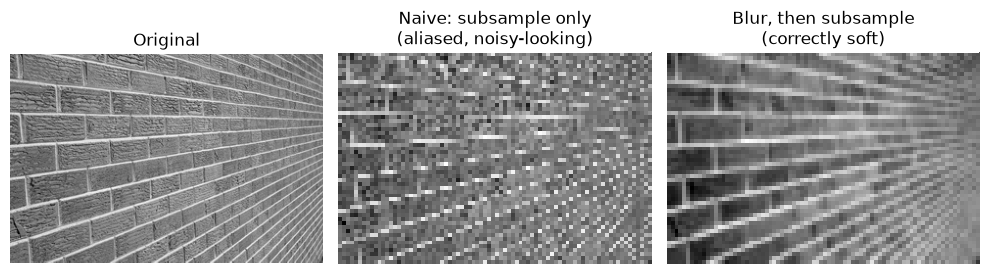
\includegraphics[width=0.95\textwidth]{figures/lesson11_fig01.png}
\caption{Naive subsampling turns the regular brick pattern into fine, noise-like speckle --- a classic aliasing artifact (the same effect that makes a car's wheels look like they're spinning backwards on camera). Blurring first keeps the wall recognizable. \attrib{Photo: \href{https://www.publicdomainpictures.net/}{publicdomainpictures.net}.}}
\label{fig:l11-1}
\end{figure}

\section{Choosing sigma and kernel size}

Blurring correctly before downsampling needs two things: the right \code{sigma}, and a kernel \emph{large enough to represent that sigma}. Concretely, blurring a single pixel with a $3\times3$ Gaussian kernel is nothing more than a weighted average of its $3\times3$ neighborhood. For \code{sigma=1.0}, the manual weighted-sum computation matches \code{cv2.GaussianBlur}'s output for that pixel exactly (up to integer rounding: $139.40$ manually vs.\ $139$ from OpenCV). Figure~\ref{fig:l11-2} shows the effect of sigma at several values.

\begin{figure}[h]
\centering
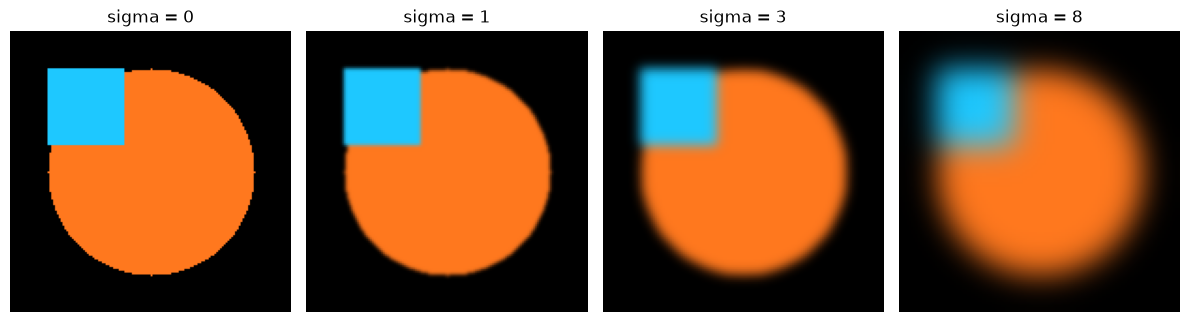
\includegraphics[width=0.95\textwidth]{figures/lesson11_fig02.png}
\caption{Larger sigma averages over a wider neighborhood, removing finer detail, as long as the kernel is large enough to represent it.}
\label{fig:l11-2}
\end{figure}

\subsection*{Kernel size has to keep up with sigma}

\code{cv2.getGaussianKernel} always renormalizes its weights to sum to 1, no matter how few taps it's given --- so a too-small kernel doesn't just clip the Gaussian's tails, it silently reshapes the whole kernel into something close to a plain box average. A 3-tap kernel built for \code{sigma=5.0} comes out as $[0.331,\ 0.338,\ 0.331]$ --- nearly identical to a plain box average $[0.33,0.33,0.33]$, the wide bell curve squashed away entirely (Figure~\ref{fig:l11-3}).

\begin{figure}[h]
\centering
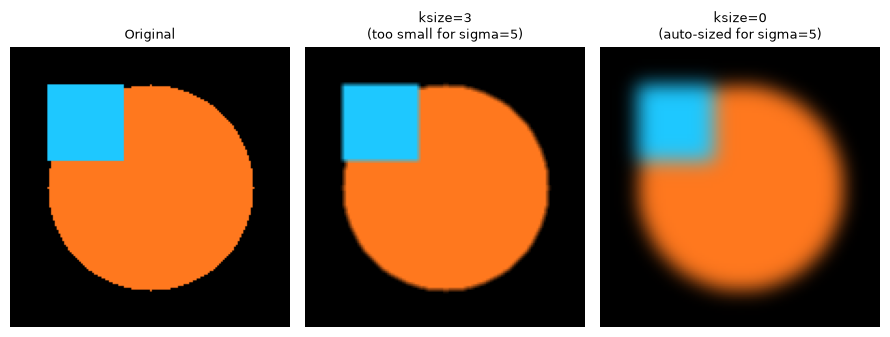
\includegraphics[width=0.85\textwidth]{figures/lesson11_fig03.png}
\caption{A $3\times3$ kernel is far too small to represent \code{sigma=5}: mean absolute difference against the correctly auto-sized kernel is $9.31$ gray levels.}
\label{fig:l11-3}
\end{figure}

This is exactly why the pyramid code below (and the aliasing fix above) passes \code{ksize=(0, 0)}: letting OpenCV choose a kernel wide enough for the requested sigma, rather than risking a silently-too-small one.

\section{Building a Gaussian pyramid}

A \textbf{Gaussian pyramid} repeats ``blur, then downsample by 2'' over and over, producing a stack of images each half the width and height of the previous one. Each level is a properly anti-aliased, coarser view of the same scene --- not just a smaller crop.

\begin{lstlisting}
def gaussian_pyramid(image, num_levels, sigma=1.0):
    pyramid = [image]
    current = image
    for _ in range(num_levels - 1):
        blurred = cv2.GaussianBlur(current, (0, 0), sigmaX=sigma)
        current = blurred[::2, ::2]
        pyramid.append(current)
    return pyramid
\end{lstlisting}

Figure~\ref{fig:l11-4} shows the resulting pyramid.

\begin{figure}[h]
\centering
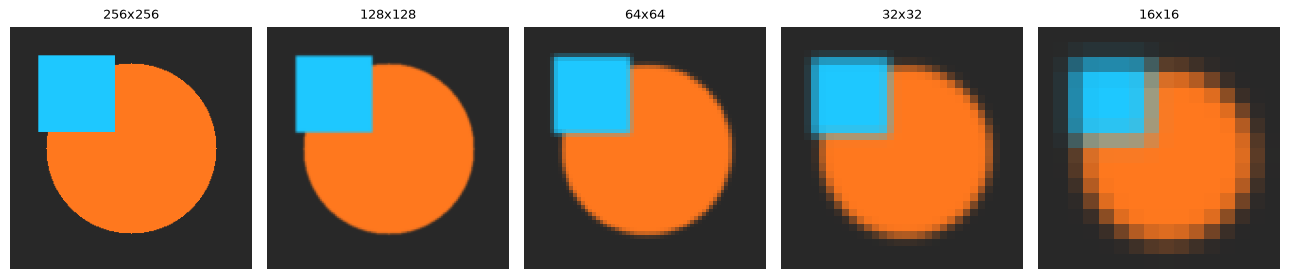
\includegraphics[width=0.95\textwidth]{figures/lesson11_fig04.png}
\caption{A 5-level Gaussian pyramid: $256\times256$ down to $16\times16$.}
\label{fig:l11-4}
\end{figure}

\subsection*{Comparison to OpenCV's built-in \code{cv2.pyrDown}}

OpenCV provides \code{cv2.pyrDown}, which does the same blur-then-downsample idea using a fixed, carefully designed 5-tap binomial kernel (approximating a Gaussian) instead of an arbitrary sigma. The output sizes match ours exactly; pixel values are close but not identical, since the kernels differ slightly --- mean absolute difference grows from $0.00$ at the original size to just $0.19$ at $16\times16$.

\section{Pyramids lose information}

Downsampling is not reversible: upsampling a lower pyramid level back to the original size (\code{cv2.pyrUp}) cannot recover detail that blurring/subsampling discarded. This gap between an upsampled coarse level and the original is exactly what a \textbf{Laplacian pyramid} captures at each level (Chapter~\ref{ch:lesson13}), but the information loss is already visible directly, in Figure~\ref{fig:l11-5}.

\begin{figure}[h]
\centering
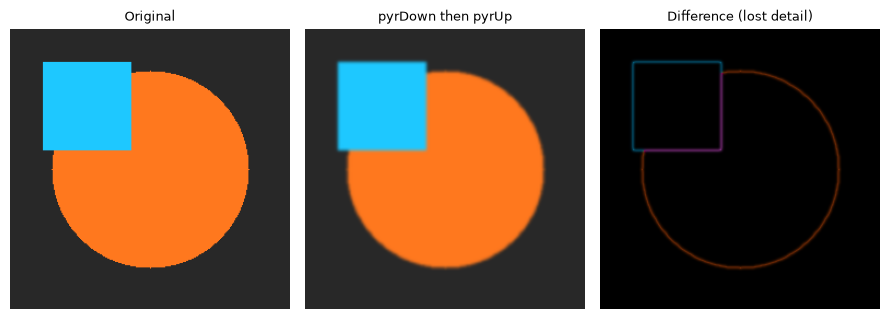
\includegraphics[width=0.85\textwidth]{figures/lesson11_fig05.png}
\caption{\code{pyrDown} then \code{pyrUp} loses detail permanently: mean absolute reconstruction error is $1.59$ gray levels. The sharp edges of the circle and square come back soft and shifted-looking --- \code{pyrUp} (interpolation) can only guess, not restore, the discarded detail.}
\label{fig:l11-5}
\end{figure}

\subsection*{Exercises}
\begin{enumerate}
  \item Repeat the brick-wall experiment with \code{factor = 2} instead of \code{4}. Does naive subsampling still show visible aliasing? Why might a smaller downsampling factor alias less?
  \item Gaussian pyramids are used for coarse-to-fine search (e.g.\ quickly finding an approximate object location at a small pyramid level, then refining at larger levels). Why would skipping the blur step and just subsampling directly break this strategy?
  \item Build a 6-level pyramid of a real photo-like image and measure how many levels it takes before the image becomes too small to recognize any shape at all. What real-world resolution would that correspond to for, say, a $1920\times1080$ photo?
\end{enumerate}

\vfill
\fullcode{lesson11}{lesson11_smoothing_pyramids}
